\documentclass[10pt,a4paper]{article}
\usepackage[utf8]{inputenc} % para poder usar tildes en archivos UTF-8
\usepackage[spanish]{babel} % para que comandos como \today den el resultado en castellano
\usepackage{a4wide} % márgenes un poco más anchos que lo usual
\usepackage[conEntregas]{caratula}
\usepackage{amssymb}
\usepackage{amsthm}
\usepackage{fancybox}
\usepackage[usenames,dvipsnames]{color}
\usepackage{hyperref}
\usepackage{listings}
\usepackage{ulem}
\usepackage{color}
\usepackage[table]{xcolor}
\usepackage{amsmath}
\usepackage{float}
\usepackage{pdflscape}
\usepackage{pdfpages}
%\usepackage[landscape]{geometry}
\usepackage{pdfpages}
\usepackage{algorithm}
\usepackage{algorithmic}
\floatname{algorithm}{Algoritmo}
\renewcommand{\listalgorithmname}{Lista de algoritmos}
\renewcommand{\algorithmicrequire}{\textbf{Entrada:}}
\renewcommand{\algorithmicensure}{\textbf{Salida:}}
\renewcommand{\algorithmicend}{\textbf{fin}}
\renewcommand{\algorithmicif}{\textbf{si}}
\renewcommand{\algorithmicthen}{\textbf{entonces}}
\renewcommand{\algorithmicelse}{\textbf{si no}}
\renewcommand{\algorithmicelsif}{\algorithmicelse,\ \algorithmicif}
\renewcommand{\algorithmicendif}{\algorithmicend\ \algorithmicif}
\renewcommand{\algorithmicfor}{\textbf{para}}
\renewcommand{\algorithmicforall}{\textbf{para todo}}
\renewcommand{\algorithmicdo}{\textbf{hacer}}
\renewcommand{\algorithmicendfor}{\algorithmicend\ \algorithmicfor}
\renewcommand{\algorithmicwhile}{\textbf{mientras}}
\renewcommand{\algorithmicendwhile}{\algorithmicend\ \algorithmicwhile}
\renewcommand{\algorithmicloop}{\textbf{repetir}}
\renewcommand{\algorithmicendloop}{\algorithmicend\ \algorithmicloop}
\renewcommand{\algorithmicrepeat}{\textbf{repetir}}
\renewcommand{\algorithmicuntil}{\textbf{hasta que}}
\renewcommand{\algorithmicprint}{\textbf{imprimir}} 
\renewcommand{\algorithmicreturn}{\textbf{devolver}} 
\renewcommand{\algorithmictrue}{\textbf{cierto }} 
\renewcommand{\algorithmicfalse}{\textbf{falso }} 


\hypersetup{
    colorlinks,
    citecolor=black,
    filecolor=black
    linkcolor=black,
    urlcolor=black
}

\lstdefinestyle{customc}{
  belowcaptionskip=1\baselineskip,
  breaklines=true,
  frame=L,
  xleftmargin=\parindent,
  language=C,
  showstringspaces=false,
  basicstyle=\footnotesize\ttfamily,
  keywordstyle=\bfseries\color{green!40!black},
  commentstyle=\itshape\color{purple!40!black},
  identifierstyle=\color{blue},
  stringstyle=\color{orange},
}

\newtheorem{theorem}{Teorema}[section]
\newtheorem{corollary}{Corolario}[theorem]
\newtheorem{lemma}[theorem]{Lema}
\newtheorem{definition}[theorem]{Definicion}

\newcommand{\norm}[1]{\left\lVert#1\right\rVert}

\newcommand{\BigO}[1]{\ensuremath{\operatorname{O}\bigl(#1\bigr)}}
\newtheorem{proposition}{Proposici\'on}

\begin{document}

\titulo{Segundo parcial}

\fecha{\today}

\materia{Algoritmos y Estructuras de Datos Avanzadas}

\integrante{Vileriño, Silvio}{106/12}{svilerino@gmail.com}

\maketitle

\tableofcontents
\newpage

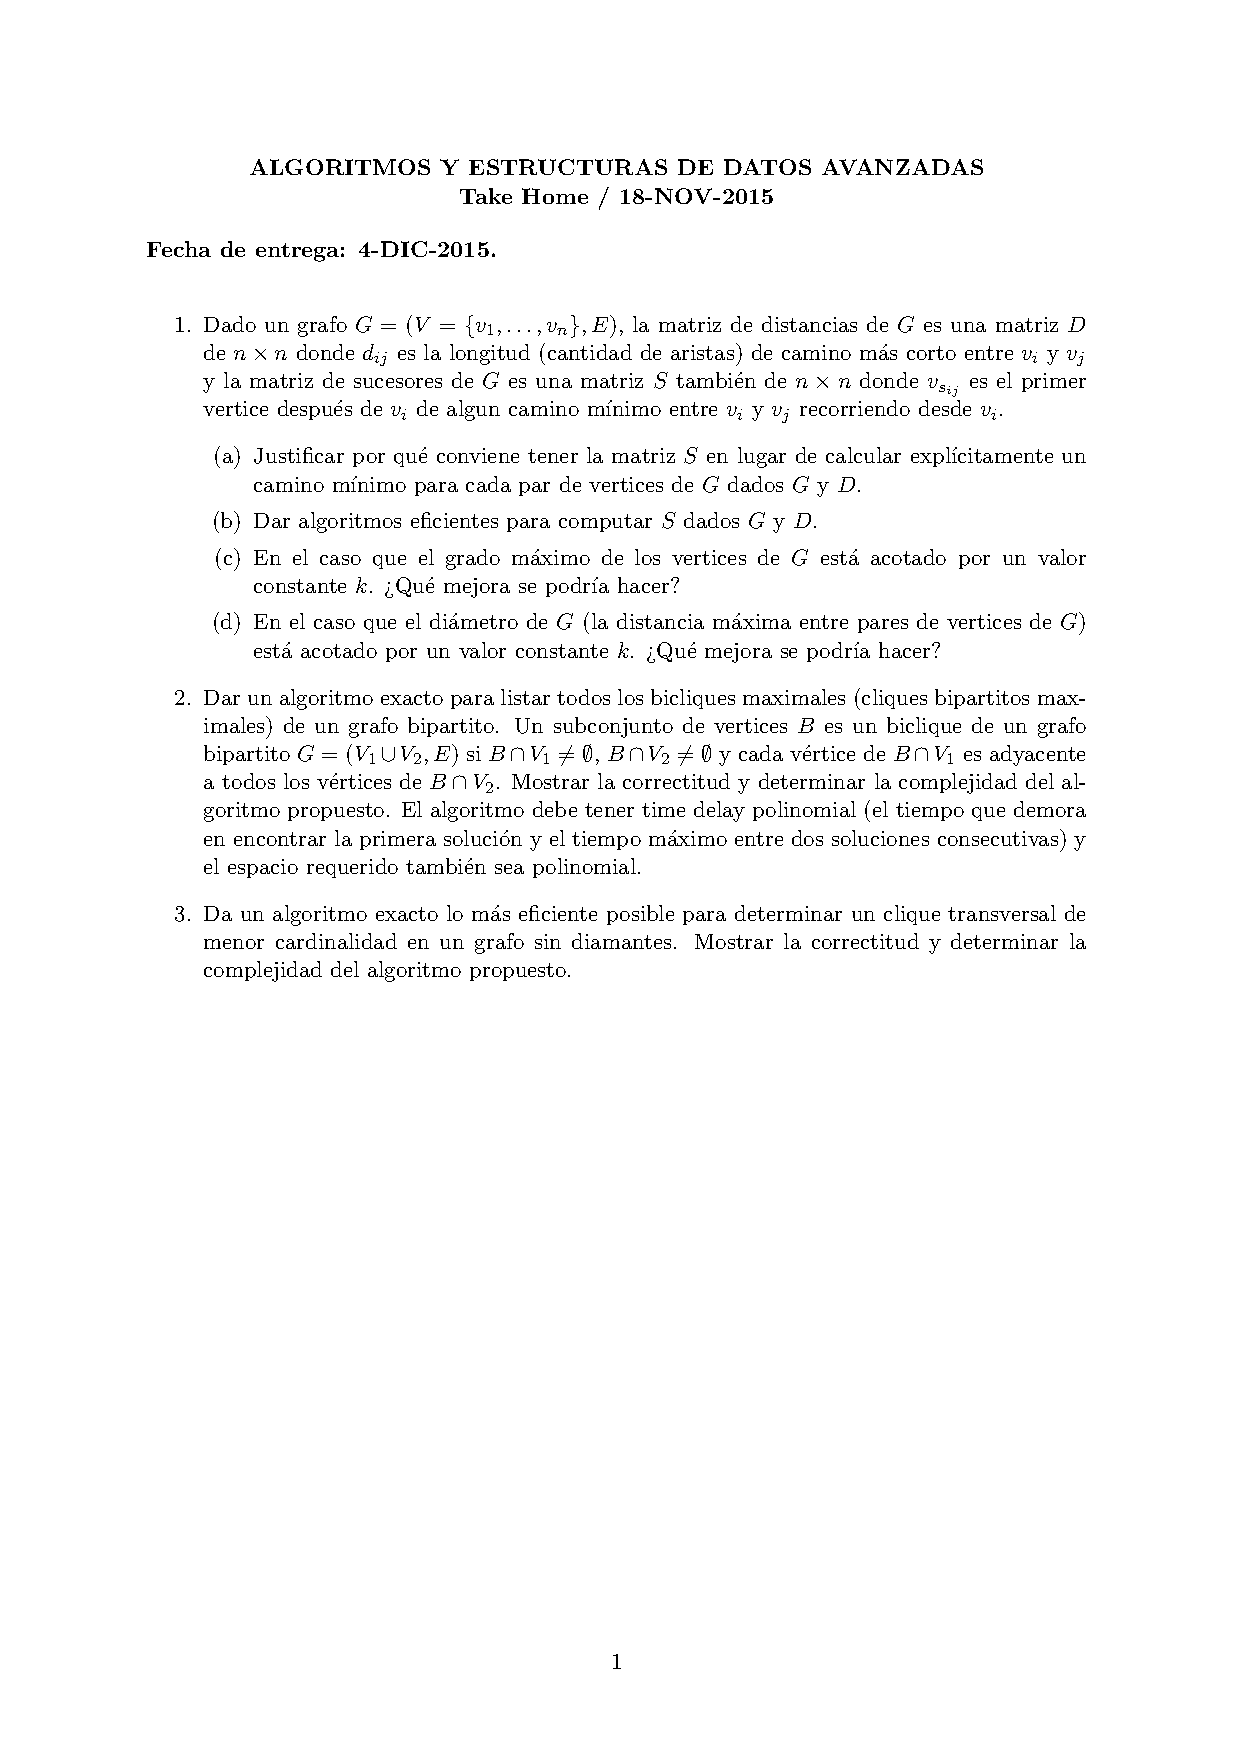
\includepdf[pages={1}]{take-home18112015.pdf}

\newpage

\section{Ejercicio 1}

\subsection{Item a)}

Desde el punto de vista de la complejidad espacial, si almacenamos todos los caminos mínimos, esto tiene un costo espacial de $\mathcal{O}(n^3)$ y el costo de devolver un camino es de tiempo constante $\mathcal{O}(1)$. Por otro lado, utilizando la matriz de sucesores S, podemos devolver un camino mínimo entre cualquier par de nodos con complejidad temporal $\mathcal{O}(n)$ y espacial $\mathcal{O}(n^2)$. El hecho de tener la matriz S constituye una mejora sustancial en el espacio asintótico consumido, por lo tanto resulta mas conveniente. A continuación presentamos el pseudocódigo de un algoritmo para calcular camino mínimo entre un par de nodos i, j dada la matriz S:

\begin{algorithm}[H]
	\begin{algorithmic}[1]
		\REQUIRE Matriz S, nodos i, j
		\ENSURE Camino mínimo entre los nodos i, j
		
		\STATE path = $\emptyset$
		\WHILE {i $\neq$ j}
		    \STATE path.append(i)
		    \STATE i = S[i][j]
		\ENDWHILE
		\STATE path.append(i) //Ultimo nodo del camino
		\RETURN path
		
	\end{algorithmic}
	\caption{Camino mínimo entre 2 nodos utilizando la matriz de sucesores S}\label{alg:alg1a}
\end{algorithm}

\subsection{Item b)}

Para el cálculo de la matriz de sucesores S en base a G y D, proponemos dos enfoques:\\
El primer enfoque consiste en utilizar el algoritmo visto en clase, que utiliza un algoritmo randomizado para calcular las matrices de testigos. La matriz S se calcula a partir de las matrices de testigos de tres productos matriciales. El costo de calcular S de esta manera, es, en promedio, $\mathcal{O}(M(n) * log(n)^2)$, donde $M(n)$ corresponde al costo temporal de la multiplicacion matricial, actualmente es $\mathcal{O}(n^{2.376})$.\\
\newline
El segundo enfoque, se basa en la idea de iterar sobre cada par de vertices (i,j) y computar $S_{i,j}$. El cómputo de $S_{i,j}$ es como sigue: miramos cada vecino k del nodo i, si vale $D_{i,j} = D_{i,j} - 1$ entonces actualizamos al nodo k como el sucesor en el camino mínimo entre los nodos i, j. Con esta idea en mente, se presenta el siguiente pseudocódigo:

\begin{algorithm}[H]
	\begin{algorithmic}[1]
		\REQUIRE Grafo G, matriz de distancias D
		\ENSURE Matriz de sucesores de caminos mínimos S
		
	    \FOR {$i=1$ hasta $n$}
    	    \STATE $Vec_i$ = Vecinos del nodo i;
	    \ENDFOR
		
		\FOR {$i=1$ hasta $n$}
    		\FOR {$j=1$ hasta $n$}
    		    \FORALL{k $\in$ $Vec_i$ }
    		        \IF{$D_{k,j} = D_{i,j} - 1$}
    		            \STATE $S_{i,j} = k$;
    		            \STATE break;
    		        \ENDIF
    		    \ENDFOR
    		\ENDFOR
		\ENDFOR
		
	\end{algorithmic}
	\caption{Construcción de la matriz de sucesores S}\label{alg:alg1b}
\end{algorithm}

Calculemos la complejidad del algoritmo \ref{alg:alg1b} propuesto:
\begin{itemize}
    \item $\mathcal{O}(n^2)$ de la inicialización de la matriz S
    \item $\mathcal{O}(n^2)$ de la inicialización de las vecindades de los nodos.
    \item El costo de los ciclos anidados es $\displaystyle\sum_{i=1}^{n} \sum_{j=1}^{n} Vec_i = n*\sum_{i=1}^{n} Vec_i = n*m $
\end{itemize}

Constituyendo un costo asintotico temporal total de $\mathcal{O}(n^2 +n*m)$.

\subsection{Item c)}
Dada esta precondición, resulta que al ser el grado constante, entonces m = O(n). Si utilizamos el algoritmo \ref{alg:alg1b}, ahora su costo temporal asintótico pasa a ser $\mathcal{O}(n^2)$.

\subsection{Item d)}
En este caso, tenemos que el diámetro es una constante k. Esto implica que todos los caminos mínimos pasan a tener longuitud constante. Si volvemos al tradeoff presentado en el item a), bajo esta precondición, almacenar los caminos mínimos precalculados, pasa a costar $\mathcal{O}(n^2)$ espacialmente, con lo cual utilizar la matriz S, carece de sentido.

\section{Ejercicio 2}
\subsection{Correctitud}

\begin{proposition}
Sean $G = ( V = V_1 \cup V_2, E)$ un grafo bipartito, $C \subseteq V$ un subconjunto de vertices tal que $ C \neq V_1 \land C \neq V_2 $ y $G' = (V = V_1 \cup V_2, E')$ con aristas adicionales tal que $V_1$ y $V_2$ sean cliques. Entonces el subgrafo inducido por C es clique maximal en G' si y solo si el subgrafo inducido por C es biclique maximal en G.
\end{proposition}

\begin{proof}
$\Rightarrow)$

Sea $ C \neq V_1 \land C \neq V_2 $ clique maximal de G'. Supongamos que C no es biclique de G. \footnote{Recordemos que G es el grafo G' sin las aristas adicionales para forzar que $V_1$ y $V_2$ sean cliques en G'.} Entonces existe al menos un nodo $v \in C \cap V_1(G)$ \footnote{An\'alogamente $v \in C \cap V_2(G)$} que no es adyacente a al menos un nodo de $C \cap V_2(G)$\footnote{An\'alogamente $C \cap V_1(G)$}. Pero observemos entonces, que si volvemos a agregar las aristas que clausuran $V_1$ y $V_2$ conformando G', entonces C no es una clique de G', lo cual contradice la hip\'otesis, y es absurdo.\\

Ahora supongamos que la biclique C no es maximal, luego existe un nodo $w \notin C$ tal que es adyacente a todos los nodos $v \in C$ de forma tal que adem\'as estos nodos $v$ pertenezcan al conjunto independiente contrario al cual pertenece $w$. Dicho esto, tenemos que w tiene intersección en $G'$ con todos los nodos pertenecientes a su partición\footnote{Conjunto independiente V1 o V2} pues agregamos esos ejes al clausurar G. Por otro lado, interseca con todos los nodos pertenecientes a C tal que estan en la particion contraria. Esto implica que entonces C no es maximal en G', lo cual es absurdo por hipótesis. 
\end{proof}

\begin{proof}
$\Leftarrow)$

Sea $ C \neq V_1 \land C \neq V_2 $ biclique maximal en G. Supongamos que C no es clique en G'\footnote{Recordemos que G' es el grafo G con las aristas adicionales para forzar que $V_1$ y $V_2$ sean cliques.}. Entonces debe faltar una arista $e$ que tiene un extremo en cada conjunto $V_1(G')$ y $V_2(G')$ porque $V_1(G')$ y $V_2(G')$ son cliques por construcci\'on. Con lo cual tampoco C es biclique en G, contradiciendo la hip\'otesis, absurdo.\\

Ahora supongamos que C no es clique maximal en G', luego existe un nodo $j \notin C$ que es adyacente a todo otro vértice de C en G'. Podemos entonces decir que $j \notin C$ en G y es adyacente a todos los vertices del conjunto independiente contrario en G, luego C no es biclique maximal en G, lo cual contradice la hipotesis.  
\end{proof}

Con estos dos resultados, planteamos la correctitud de la equivalencia entre buscar cliques maximales sobre G' y buscar bicliques maximales sobre G. Mostrando que nuestro algoritmo es correcto, mas aun, al devolver el resultado, se verifica(en tiempo polinomial) que no se estan devolviendo las cliques ficticias agregadas a G'.

\subsection{Algoritmo propuesto}

\begin{proposition}[Visto en clase - Tsukiyama]
Sea $G = (V, E)$ un grafo, existe un algoritmo para listar todos los cliques maximales con las siguientes propiedades:
\begin{itemize}
    \item Complejidad espacial: $\mathcal{O}(n + m)$
    \item Time delay: $\mathcal{O}(n*m)$
\end{itemize}
\end{proposition}

Sea $G = ( V = V_1 \cup V_2, E)$ un grafo bipartito, existe un algoritmo para listar todas los bicliques maximales de G utilizando el algoritmo mencionado en la proposición anterior. La idea del mismo es como sigue:

\begin{enumerate}
    \item Entrada: $G = ( V = V_1 \cup V_2, E)$ un grafo bipartito.\footnote{Sin perdida de generalidad consideramos este grafo tal que si numeramos los nodos, los que pertenezcan al conjunto independiente $V_1$ preceden a los que pertenezcan a $V_2$}
    \item Precomputar los conjuntos independientes de nodos $V_1$ y $V_2$ de G.
    \item Construir $G' = (V = V_1 \cup V_2, E')$ adicionando aristas a los conjuntos independientes $V_1$ y $V_2$ para que sean cliques.
    \item Correr el algoritmo para listar cliques maximales sobre G'.
    \item Revisar el primer resultado del algoritmo de Tsukiyama
    \begin{enumerate}
        \item Si este primer output tiene interseccion vacía respecto de $V_1(G')$ o $V_2(G')$, ignorar el resultado y continuar con el algoritmo.
        \item Caso contrario, devolverlo como un resultado valido. 
    \end{enumerate}
    \item Para cada resultado T obtenido con el algoritmo luego de la primera, considerar los siguientes dos casos:
    \begin{enumerate}
        \item Si T intersecta con $V_1(G')$ y con $V_2(G')$ de forma no vacia, considerarlo un resultado valido y continuar con el algoritmo.
        \item Caso contrario, terminar el algoritmo.
    \end{enumerate}
\end{enumerate}

Dado el ordenamiento de nodos que proponemos para la entrada G, resulta que si $V_1$ o $V_2$ son cliques maximales, estas serán devueltas al principio y al final del algoritmo respectivamente. Esto indica que nuestros chequeos al principio de descarte del primer resultado y nuestra condicion de corte del algoritmo, son medidas licitas para garantizar correctitud. Por otro lado, dado que en nuestro algoritmo propuesto devolvemos conjuntos que cumplen las hipótesis de los resultados demostrados en la seccion anterior, y hemos establecido una equivalencia entre cliques y bicliques maximales de G y G'. El algoritmo que se propuso se puede considerar correcto.

\newpage

\subsection{Complejidad}

La operacion de clasificacion del grafo en particiones $V_1$ y $V_2$ puede ser resuelta mediante un algoritmo de exploracion\footnote{Por ejemplo DFS o BFS} de grafos y utilizando una estructura de consulta dinamica\footnote{Por ejemplo una tabla hash o un arreglo}, esto es claramente polinomial. Por otro lado, la clausura del grafo G' puede realizarse en tiempo polinomial.


Respecto a la complejidad espacial, notemos que agregar aristas al grafo G para construir G' consume espacio polinomialmente. Por otro lado, el algoritmo propuesto, consume espacio polinomialmente, con lo cual el espacio total ocupado es polinomial.\\

Respecto al time delay polinomial, clausurar V1 y V2 para el preprocesamiento es temporalmente polinomial y el algoritmo presentado tiene time delay polinomial, entonces si el preprocesamiento es polinomial y correr el algoritmo sobre G' es polinomial, el tiempo de espera hasta el primer resultado es polinomial. Por otro lado, el tiempo de espera entre resultados no cambia, pues es el time delay intr\'inseco del algoritmo que se vi\'o en clase y revisar que las cliques devueltas no correspondan a las cliques espurias generadas en G' sobre $V_1$ y $V_2$ tambien consume tiempo polinomial.

\section{Ejercicio 3}
\subsection{Resultados auxiliares y algoritmo propuesto}
Comenzaremos con algunos resultados teóricos y luego propondremos un algoritmo para la resolución de este problema.

\begin{proposition}
    Sea G diamond-free entonces toda arista pertenece a lo sumo a una clique. \textbf{Esta propiedad fue vista en clase}.
\end{proposition}

\begin{proposition}
    Sea G diamond-free, sin nodos aislados, entonces a lo sumo tiene m cliques.
\end{proposition}
\begin{proof}
    Pensemos combinatoriamente el problema, establezcamos una analogía entre cliques como cajas y aristas como bolitas.\\
    Como por hipótesis no existen nodos aislados, luego toda clique tiene al menos una arista, o análogamente, toda caja tiene al menos una bolita.\\
    Por la proposición anterior vista en clase, cada arista está en una sola clique, o análogamente, cada bolita puede solo ir a parar a una sola caja.\\
    Finalmente, concluimos que si toda caja tiene alguna bolita, entonces tiene que haber mas bolitas que cajas. Análogamente, en términos del problema, se tiene que  \#(cliques de G) = \#(cajas) $\leq$ \#(bolitas) = m. 
\end{proof}

\begin{proposition}
Sea G diamond-free, entonces tiene a lo sumo n + m cliques.
\end{proposition}
\begin{proof}
Consideremos al grafo G tal que tenga n nodos aislados, que son cliques. Luego sea G' = G $\setminus$ $\{$ nodos aislados $\}$. Por la proposición anterior, G' tiene a lo sumo m cliques. Totalizando que G tiene a lo sumo n+m cliques.
\end{proof}

Con estos resultados se propone la siguiente idea:
\begin{itemize}
    \item Se calculan todas las cliques de G (\textbf{Con el algoritmo visto en clase}).
    \item Se prueban todos los posibles subconjuntos de nodos posibles, en particular, todos los conjuntos clique transversales).
    \item Se filtra el subconjunto  de cardinalidad mínima que tenga interseccion no vacía respecto de todas las cliques.
\end{itemize}
A continuación se presenta el pseudocódigo que ilustra esta idea:

\begin{algorithm}[H]
	\begin{algorithmic}[1]
		\REQUIRE Grafo G
		\ENSURE W clique transversal de cardinal mínimo

        \STATE Sean $\{C_i\}_{i \in \mathbb{N}} = \{$ Cliques de G $\}$ // Calcular con algoritmo visto en clase
        \STATE Sea k = $\#\{C_i\}$ // Cantidad de cliques de G
    
		\FOR {$i=1$ hasta $n$}
		    \FORALL{W $\subseteq$ $V(G)$ tal que $\#W = i$ }
		        \IF{$W \cap C_k \neq \emptyset $ $ \forall$ $ C_1, \dots, C_k$}
		            \RETURN W;
		        \ENDIF
		    \ENDFOR
		\ENDFOR
		
	\end{algorithmic}
	\caption{Clique transversal de cardinal mínimo en grafo sin diamantes}\label{alg:alg3}
\end{algorithm}

\subsection{Correctitud}
Este algoritmo realiza lo que se mencionó en la idea mas arriba y es correcto, pues se prueban todos los posibles conjuntos clique transversal, de menor a mayor en cardinalidad, al encontrar el primero y devolverlo finalizando el algoritmo, esto asegura que sea uno de cardinal mínimo.

\subsection{Complejidad}
Analicemos con un poco de cuidado, la complejidad total del algoritmo \ref{alg:alg3}.
\begin{itemize}
    \item El cálculo de las cliques del grafo G tiene un costo temporal de $\mathcal{O}(\alpha(G)*m + n^2)$ donde $\alpha(G)$ es la arboricidad del grafo G. \textbf{Algoritmo visto en clase}.
    \item Por otro lado, el costo temporal de los ciclos anidados es $\displaystyle\sum_{i} \binom{n}{i} * (n + m) * n$, pues para cada i, existen $\binom{n}{i}$ subconjuntos de i nodos, por otro lado, para cada subconjunto W, hay que corroborar que la interseccion no sea nula para todas las cliques $C_1, \dots, C_k $ del grafo G.\\
    Por la proposición vista anteriormente, k = O(n + m) y como cada clique tiene O(n) elementos, ver si la interseccion es no nula contra cada una ellas cuesta O(n). Esto se repite $\beta(G)$ veces, donde $\beta(G)$ indica el cardinal del clique transversal mínimo del grafo G. Más formalmente se tiene que el costo del algoritmo es:\\
    \begin{itemize}
        \item $\mathcal{O}(\displaystyle\sum_{i = 1}^{\beta(G)} \binom{n}{i} * (n + m) * n)$
        \item $= \mathcal{O}((n + m) * n * \displaystyle\sum_{i = 1}^{\beta(G)} \binom{n}{i})$
        \item $= \mathcal{O}((n + m) * n * \displaystyle\sum_{i = 1}^{\beta(G)} \frac{n^i}{i!})$
        \item $= \mathcal{O}((n + m) * n * n^{\beta(G)})$
    \end{itemize}
    
A este último resultado se le debe sumar el $\mathcal{O}(\alpha(G)*m + n^2)$ del calculo de las cliques de G. Entonces, El costo temporal total es:

$\mathcal{O}(\alpha(G)*m + n^2 + (n + m) * n * n^{\beta(G)})$, pero como estamos trabajando con complejidad asintótica y vale que $\alpha(G) \leq m$, \textbf{finalmente resulta $\mathcal{O}((n + m) * n * n^{\beta(G)})$}.
    
\end{itemize}

\end{document}
